%\documentclass[10pt,a4paper,twoside,draft]{report}
\documentclass[10pt,a4paper,twoside]{report}
%\usepackage{lipsum}
\usepackage[latin1]{inputenc}
%\usepackage[dutch]{babel}
\usepackage{babel}
\usepackage{datetime2}
\usepackage{graphicx}
\usepackage{makeidx}
\usepackage{array}
\usepackage{tikz}
\usepackage{xparse,nameref}
\usepackage[columns=2,indentunit=10pt,totoc=true]{idxlayout}
%\usepackage{showidx}
\usepackage{transparent}
%\usepackage[firstpage]{draftwatermark}
%\usepackage{wrapfig}
\usepackage{url}
\usepackage[pdfpagelabels=true,plainpages=false,hyperfootnotes=false]{hyperref} % last package!
%\usepackage[final=true]{hyperref}

\newcommand{\Author}{A.H.M. Steenveld}
\newcommand{\CC}{CncCalculator}

%\SetWatermarkText{\transparent{0.1}\includegraphics[scale=0.26,angle=225]{./images/None.jpg}}

\bibliographystyle{plainnat}

\author{\Author.}
\title{
	\begin{figure}[h!]
		\centering
		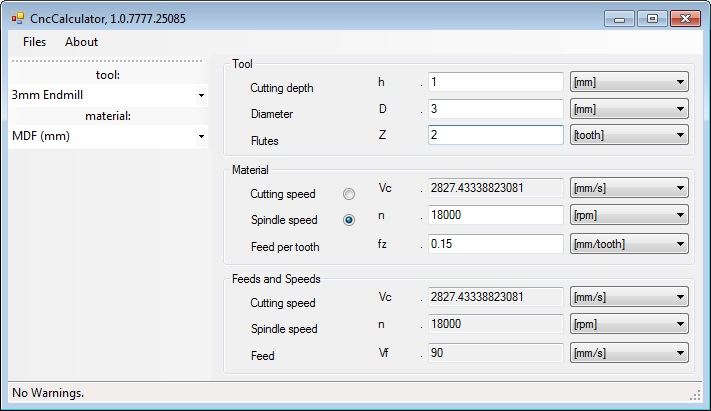
\includegraphics[width=0.6\linewidth]{../../CncCalculator_screenshot1.jpg}
	\end{figure}	
	This is your \CC.
}

\parindent=0pc			    % Do not indent the start of a paragraph.
\flushbottom				% Size all pages to the same length.
\setlength{\parskip}{1pc}	% put an empty line between paragraphs.

\makeindex
\pagestyle{empty}
\begin{document}
	\maketitle
	\pagebreak\begin{abstract}		
	Getting access to a CNC machine has become more easy over the years.
	Using such machines optimal requires some a propper configuration, a choice of the right tools
	and to do some calculations. The questions behind the most bacic calculations are `How fast should
	my spindle turn?' and `How fast can I move through the material?'
	
	The calculations involved are quite simple, with the correct information just multiply and divide
	a few values. It becomes a bit more ticky when some of the values involved are given in 
	the metric sysem and others are in the imperial system. Conversion between the unit systems is
	an area where a mistake is made easily but often spotted too late.
	
	\CC\ will do all the calculations if provided with the right information and will do
	unit conversion `on the fly' as required. In this document the calculations used are explained
	as wel as the method of conversion between the unit systems.
	
	\CC\ being what it is, a tool that helps the user, will provide you with a calculated
	result. It is still up to you to make an estimate if this is a reasonable result. For this it
	helps to have at least a look at the calulations and also on the internet for similar applications
	of tools and material to get a feeling of what a reasonale result is. In this practice is the
	teacher for good results and no tool can help you with that.
	
	This document assumes that you have some basic knowledge on what is involved in the physical process
	of cutting a part from some stock and know how to look up thinks in your machine documentation or
	on the internet. The actual process of cutting material is explained in short but not in full details.
	This is not a introduction on cutting done by a CNC machine but an explanation on how \CC\ works.
	\end{abstract}
	\pagestyle{headings}\pagenumbering{roman}
	\tableofcontents
	\listoffigures
	\newpage\pagenumbering{arabic}\setcounter{page}{1}%
	\chapter{Introduction}
	\CC\ is a tool to quickly calculate feeds and speeds born out of necesity. Too often I made a mistake
	in the calculations (or conversion) involved. ON the internet (or in the store for your smart phone) 
	more than one tool can be found for doing the calculations but I never found one I was happy with.
	I decided to make one so I don't have to look for it anymore, can change it to whatever I want it to be,
	use for free and without any spam involved.
	
	\CC\ has some strong point and weak points if you comare it whith the other ones available.	
	A few of the points are listed below. You can classify it as a strong or weak point for yourself.
	\begin{itemize}
		\item All source code is available andis available under a permissive licence form.
		\item Selection of units, e.g.: [in] or [mm].
		\item Conversion of units, e.g.: from [in/min] to [mm/sec].
		\item Includes a list of materials with preset values.
		\item Includes a list of tools with preset values.
		\item Can import any FreeCAD tools library (both v0.18 or before and v0.19 or better)
		\item Where you put it on the screen there it will be the next time you start it.
		\item Easy and intuitive to use.
	\end{itemize}

    \newpage\section{Quick start}
    Assuming that you know what `Feeds' and `Speeds' are this is a quick run trough for \CC.
    
    When you start \CC\ for the first time it comes up on a default location and using default settings.
    
    You can drag the form to any location and when you close the application it wil reopen on exact 
    the location where you closed it. This is handy when you arrange your (CNC related) tools on fixed
    positions on the screen.
    
    By default, on the top you find a menu bar with entries like `file' and `about', below that is an
    tools bar. You can drag this tools bar to any side of the application, top, left, right or bottom.
    The tools bar contains two selection buttons, one for a tool and another for a material. Selecting
    one will fill in the `Tool' or `Material' section with values from the selected item. You do not
    have to select any tool or material, it is possible to use \CC\ by filling in all required information
    by typing data in the `Tool'  and `Material' section. (see below)
    
    There are two sections for input, `tool' and `material', and one for result. Working with wood it
    is common to use a recomended spinle speed, working with other materials a more accurate specification
    of the tool cutting speed is required. Selecting between the two methods is done by selecting the
    round selection button after `Cutting speed' or `Spindle speed' in the material section. The one
    not selected will be calculated from the other and a given tool diameter.
    
    Input fields are coloured white\footnote{Depending on system settings.} and calculated fields are gray.
    Next to the field with the value is a button with a list of units. For edit fields you can select
    the appropriate units for your value. No `on the fly' conversion is done, assuming that the value
    is the right value for the units you select. For calculated fields an `on the fly' conversion is
    done and the value is changed to the correct value for the units you selected.
    
	You can select any value calculated or any value in an edit field and use `copy/paste' shortcuts
	to get the values to/from the clip board. Or you could just read and type it from/into your final
	application.
	
	\chapter{CNC machines.}
	\section{Cutting material.}
	To do.
		
	\section{Calculations.}
    To do.
	
	\chapter{Unit.}
	\section{The metric system.}
	To do.
	
	\section{The imperial system.}
	bla bla bla
	
	\section {Conversions}
	To do.
	
	\chapter{\CC}
	\section{The screens explained.}
	To do.
	
	\section{How to use \CC}
\newpage\phantomsection 
\addcontentsline{toc}{chapter}{Bibliography}
%\bibliography{CncCalculator}    
\end{document}
